\documentclass[a4paper]{article}

\usepackage[T1]{fontenc}
\usepackage{titling}
\usepackage{amsmath}
\usepackage{amsfonts}
\usepackage{graphicx}
\usepackage{mathtools}
\usepackage{subfig}

\numberwithin{equation}{section}
\usepackage[numbered, framed]{matlab-prettifier}

\lstset{
	style              = Matlab-editor,
	escapechar         = ",
	mlshowsectionrules = true,
	tabsize            = 2,
}

\addtolength{\oddsidemargin}{-.875in}
\addtolength{\evensidemargin}{-.875in}
\addtolength{\textwidth}{1.75in}

\addtolength{\topmargin}{-.875in}
\addtolength{\textheight}{1.75in}

\setlength{\droptitle}{-8em}

\title{Engineering Computation Project \\ \large Modelling Wireless Communication Channels}

\author{\textbf{Wojciech Dziwulski, Mansfield College}}

\date{}

\begin{document}

\maketitle

\section{Introduction}

This report explores the properties of various orthogonal function sets and their applicability to generating fits to real-life data.

\section{Orthogonality}

Orthogonality is a crucial mathematical concept and extends from the well-known geometrical application (vectors) to the analysis of functions.
\\ \\
We can define a set of orthogonal functions $g_0, g_1, \ldots, g_n$ whose linear combination can be used to fit an arbitrary function f:
\begin{equation}f(x) = a_0 g_0(x)+a_1 g_1(x)+a_2 g_2(x)+\ldots+a_n g_n \end{equation}
\noindent We then define an inner product operation, for which, conveniently:
\begin{equation} \langle\,g_n,g_m\rangle = 0 \quad \textrm{if} \quad n \ne m \end{equation}
So that if we compute the inner product of both LHS and RHS with some arbitrary $g_k$, like:
\begin{equation} \langle\,f,g_k\rangle = a_0\langle\,g_0,g_k\rangle + a_1\langle\,g_1,g_k\rangle + \ldots + \boldsymbol{a_k\langle\,g_k,g_k\rangle} + \ldots + a_n\langle\,g_n,g_k\rangle \end{equation}
which lets us calculate the $a_k$ coefficient as:
\begin{equation} a_k = \frac {\langle\,f,g_k\rangle} {\langle\,g_k,g_k\rangle} \end{equation}
This result is crucial, as it demonstrates that the coefficients are independent of the size of the orthogonal basis used for the investigation i.e. if more functions are decided to be added, old coefficients do not have to be recomputed.
\\ \\
Investigation of orthogonal function fitting can be started with analysing the Fourier series. The set of sines and cosines making up the basis turn out to be orthogonal under integral operation over one period.
\\
Even though useful, Fourier series is quite a basic method for function fitting and will not be analysed in detail in this report. We will instead delve into the investigation of two particularly relevant orthogonal basis functions - Gram-Schmidt and Laguerre.

\section{Gram-Schmidt functions}

\subsection{Process}

The Gram-Schmidt process stems from a very simple logic for generating orthogonal functions - choosing a linearly independent basis, and adjusting the consecutive functions appropriately, making sure that every subsequent function is orthogonal to the previous one.
\\
Hence having the linearly independent basis $v_0, v_1, v_2, \ldots, v_n$ we can compute the orthogonal functions $g_0, g_1, g_2, \ldots, g_n$ using:
\begin{align}
g_0(x) &= v_0(x) \\
g_1(x) &= v_1(x) - e_{10} g_0 (x) \\
g_2(x) &= v_2(x) - e_{20} g_0 - e_{21} g_1 (x) \\
g_3(x) &= v_3(x) - e_{30} g_0 - e_{31} g_1 (x) - e_{32} g_2 (x)
\end{align}

\noindent As noted before, using the orthogonality property we can now compute the e coefficients:
\begin{equation} g_n(x) = v_n(x) - e_{n0} g_0 - \ldots - \boldsymbol{e_{nm} g_m (x)} - \ldots - e_{n(n-1)} g_{n-1} (x) \end{equation}
Taking the inner products:
\begin{align}
\langle\,g_n,g_m\rangle &= \langle\,v_n,g_m\rangle - e_{n0} \langle\,g_0,g_m\rangle &- \ldots &- \boldsymbol{e_{nm} \langle\,g_m,g_m\rangle} &- \ldots &- e_{n(n-1)} \langle\,g_{n-1},g_m\rangle \\
0 &= \langle\,v_n,g_m\rangle - 0 &- \ldots &- \boldsymbol{e_{nm} \langle\,g_m,g_m\rangle} &- \ldots &- 0
\end{align}
\begin{equation} \Rightarrow e_{nm} = \frac{\langle\,v_n,g_m\rangle}{\langle\,g_m,g_m\rangle} \end{equation}
We can then divide each function by its norm (square root of its inner product with itself) in order to achieve an orthonormal set.

\subsection{Monomial basis}

The independent basis chosen is a set of monomials $v_0 = 1, v_1 = x, v_2 = x^2, \ldots, v_n=x^n$ which will be used to produce an orthogonal basis under operation $\int_{0}^{\infty} g_n g_m e^{-x} dx$.\\
We compute the polynomial coefficients by iteratively multiplying the previous orders' coefficient vectors by the e-scaling factor:

\lstinputlisting[caption={gs\_polynomials.m},label={lst:gspolynomials},firstline=32, lastline=46]{../Matlab/GramSchmidt/gs_polynomials.m}

\noindent The leading coefficient of the appropriate orthogonal polynomial is retrieved from the matrix of coefficients of the independent basis ("ones" in listing \ref{lst:gspolynomials}). Interestingly, the Gram Schmidt functions are stored as their polynomial coefficients instead of the y-values calculated over the supplied x-range. \\
The x-range used for the computation of the Gram Schmidt e factors was chosen so that the marginal improvement over the evaluation accuracy did not exceed 1 \% of the function value, and turned out to be around 70. \\ \\
All the functions were tested in the gs\_polynomials\_testbench.m file.

\section{Laguerre functions}

Laguerre polynomials are another example of an orthogonal set, under the inner product defined as:
\begin{equation} \label{laguerre_inner_product}
\langle\,L_n^{(\alpha)}, L_m^{(\alpha)}\rangle=\int_{0}^{\infty} x^{\alpha} e^{-x} L_n^{(\alpha)}(x), L_m^{(\alpha)}(x)dx = 
\begin{cases} 
      \frac{\Gamma(n+\alpha+1)}{\Gamma(n+1)} \quad \textrm{for} \quad m = n \\
      0 \quad \quad \quad \quad \quad \textrm{otherwise}
\end{cases}
\end{equation}
We are going to explore two methods of computing their coefficients and subsequently fit them to a real dataset.

\subsection{Rodrigues formula}

Using the Rodrigues formula, the n-th associated Laguerre polynomial is:
\begin{equation}
L_n^{(\alpha)}(x)=\frac{1}{n!}x^{-\alpha}e^x\frac{d^n}{dx^n}(x^{n+\alpha}e^{-x}), \quad\quad n \in \mathbb{N}, \alpha \in \mathbb{R}
\end{equation}
noting that after differentiation the $x^{-\alpha}$ and ${e^x}$ cancel out, all we have to do is calculate the coefficients of the differentiated product using the Leibniz rule:
\begin{equation}
(f \cdot g)^{(n)} = \sum_{k=1}^{n} \binom{n}{k} f^k g^{n-k}
\end{equation}
This is accomplished by first recursively calculating the $x^n$ coefficients and then calculating them by the rest of the appropriate product:

\lstinputlisting[caption={rodrigues\_laguerre.m},label={lst:rodrigueslaguerre},firstline=23, lastline=30]{../Matlab/Laguerre/rodrigues_laguerre.m}

\noindent Noting, however, that the Rodrigues formula is computationally inefficient due to the repeated calculation of the derivative coefficients, we turn onto a different method: the recursive method.

\subsection{Recursive method}

This method takes the advantage of the successive polynomial generation using the formula:
\begin{equation}
n L_n^{(\alpha)}(x) = (2n + \alpha + 1 - x) L_{n-1}^{(\alpha)}(x) - (n + \alpha - 1) L_{n-2}^{(\alpha)}(x)
\end{equation}
with:
\begin{align}
L_0^{(\alpha)}(x) &= 1 \\
L_1^{(\alpha)}(x) &= -x+\alpha+1
\end{align}
This is achieved by the fairly simple:
\lstinputlisting[caption={recursive\_laguerre.m},label={lst:recursivelaguerre},firstline=27, lastline=35]{../Matlab/Laguerre/recursive_laguerre.m}

\noindent Note the use of the \textit{circshift} function in order to simulate multiplication by the coefficient vector by the variable $x$.\\
For $\alpha = 0$ the Laguerre plots using the method above looked exactly as expected.

\subsection{Gram-Schmidt Laguerre comparison}

It is easy to note that under $alpha = 0$ the inner product operations for Laguerre and Gram-Schmidt polynomials look identical. This motivated an investigation of the similarities between the two orthogonal sets.

\begin{figure}
\centering
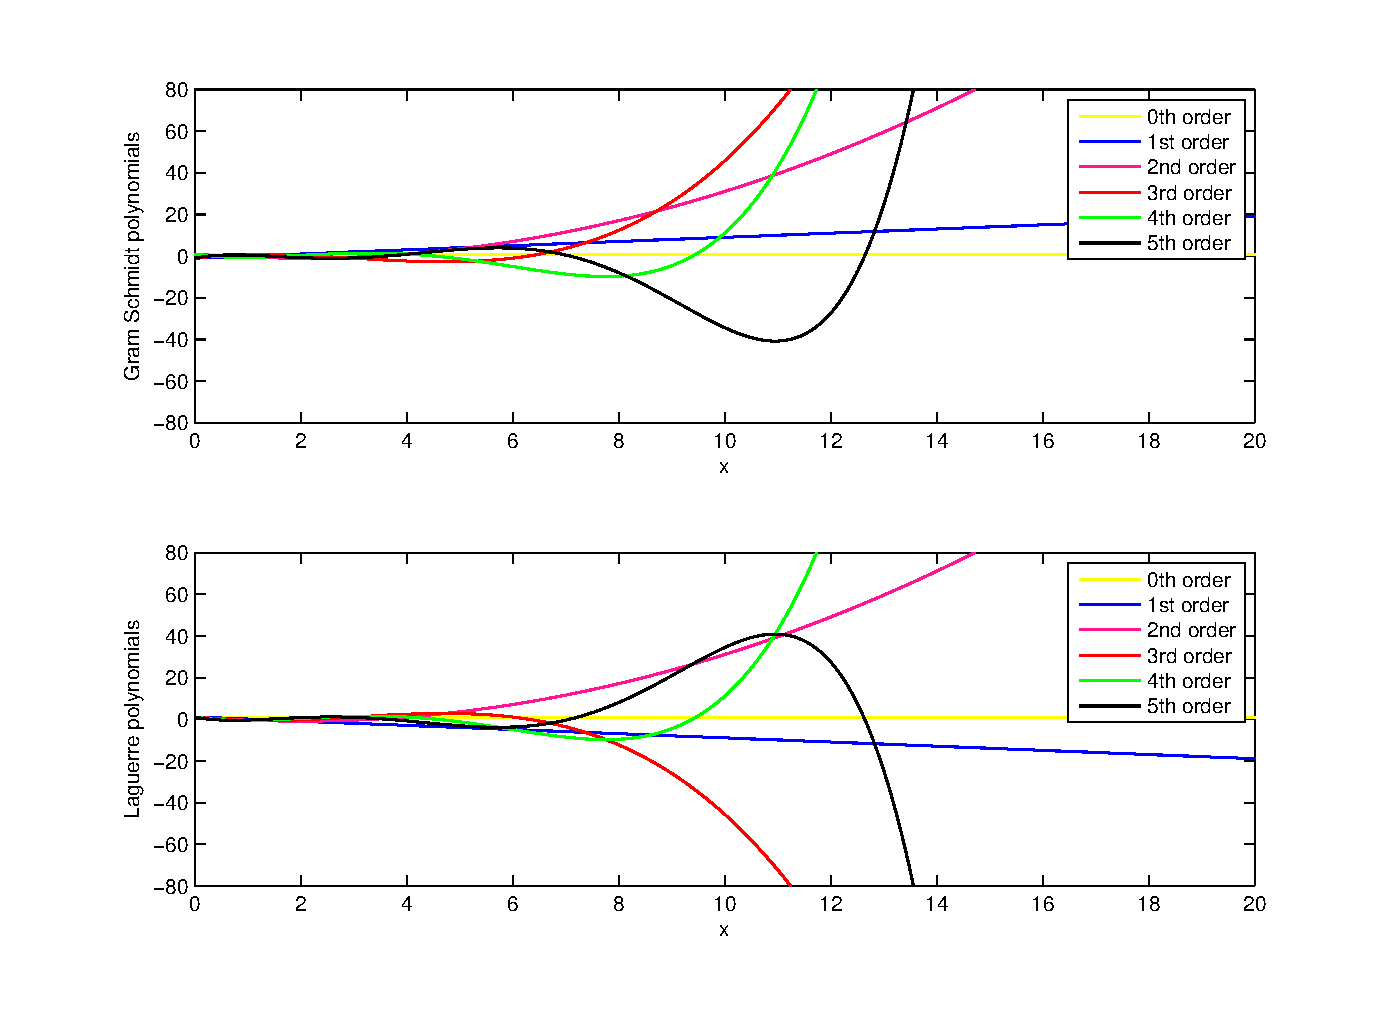
\includegraphics[width=0.8\textwidth]{gs_laguerre_comparison.eps}
\caption{\label{fig:gslaguerrecomparison}Comparison between the Gram Schmidt and Laguerre polynomials up to order 5.}
\end{figure}

When plotted side by side (Figure \ref{fig:gslaguerrecomparison}) the Gram Schmidt and Laguerre polynomials indeed turn out to have much in common. It is clear that for some of the polynomial orders, the Laguerre plot is just the Gram Schmidt plot negated. \\
This is even clearer when the polynomial coefficients for both are printed out:
\begin{align}
gs_{coefficients} &= 
\begin{pmatrix*}[r]
  0 & 0 & 0 & 0 & 0 & 1.0000 \\
  0 & 0 & 0 & 0 & 1.0000 & -1.0000 \\
  0 & 0 & 0 & 0.5000 & -2.0000 & 1.0000 \\
  0 & 0 & 0.1667 & -1.5000 & 3.0000 & -1.0000 \\
  0 & 0.0417 & -0.6667 & 3.0000 & -4.0000 & 1.0000 \\
  0.0083 & -0.2083 & 1.6667 & -5.0000 & 5.0000 & -1.0000
 \end{pmatrix*}
\\
laguerre_{coefficients} &= 
\begin{pmatrix*}[r]
  0 & 0 & 0 & 0 & 0 & 1.0000 \\
  0 & 0 & 0 & 0 & -1.0000 & 1.0000 \\
  0 & 0 & 0 & 0.5000 & -2.0000 & 1.0000 \\
  0 & 0 & -0.1667 & 1.5000 & -3.0000 & 1.0000 \\
  0 & 0.0417 & -0.6667 & 3.0000 & -4.0000 & 1.0000 \\
  -0.0083 & 0.2083 & -1.6667 & 5.0000 & -5.0000 & 1.0000
 \end{pmatrix*}
\end{align}
The odd powers of Laguerre polynomials are just their Gram Schmidt counterparts negated. This may suggest that if the linearly independent basis on which the Gram Schmidt polynomials are built is changed, both orthogonal sets are going to be equal. \\
Given that finding, it seems like negating the coefficients of odd order monomials, i.e. constructing a linearly independent set $1, -x, x^2, -x^3, \ldots$ will produce Gram Schmidt coefficients identical to the Laguerre ones. This is also algebraically consistent with the formula for Gram Schmidt coefficients and yielded expected results when implemented in MATLAB. \\
\\
Finally, the set of \textbf{associated} Laguerre polynomials was produced using the formula:
\begin{equation} \label{associated_laguerre_definition}
\psi_n^{(\alpha)}(x) = \sqrt{\frac{\Gamma(n+1)}{\Gamma(n+\alpha+1)}} x^{\alpha/2} e^{-x/2} L_n^{(\alpha)}(x)
\end{equation}
Associated Laguerre functions form an orthonormal set under the inner product \begin{equation} \label{inner_product}
\langle\,f_n, f_m \rangle = \int_{0}^{\infty}f_n(x)f_m(x)
\end{equation}
since after some algebraic manipulation it becomes analogous to the product in the equation \ref{laguerre_inner_product} with the square root factor cancelled out.

\begin{figure}[!ht]
  \centering
  \subfloat[][]{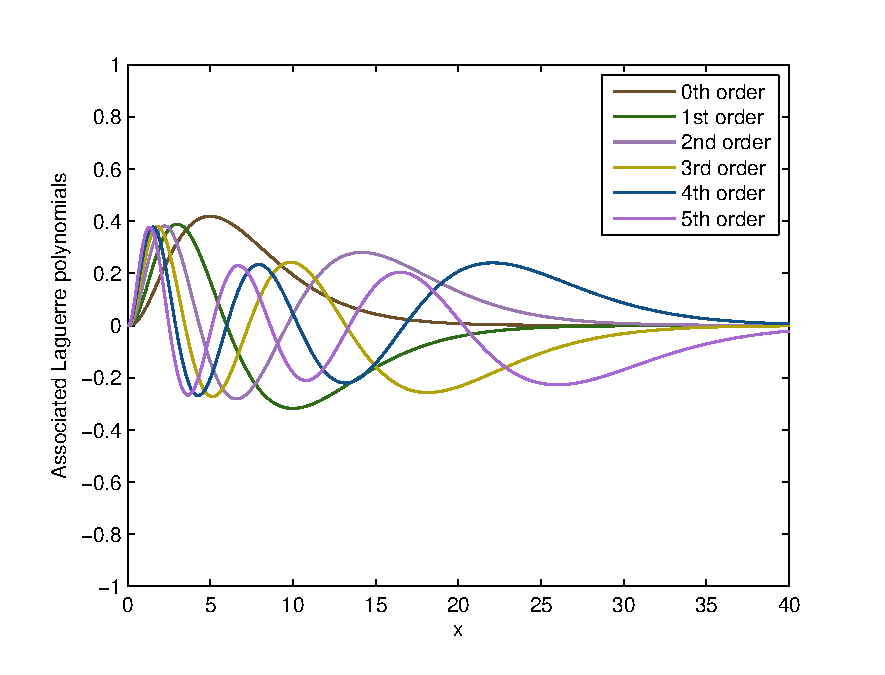
\includegraphics[width=.45\textwidth]{associated_laguerre_alpha5.eps}}\quad
  \subfloat[][]{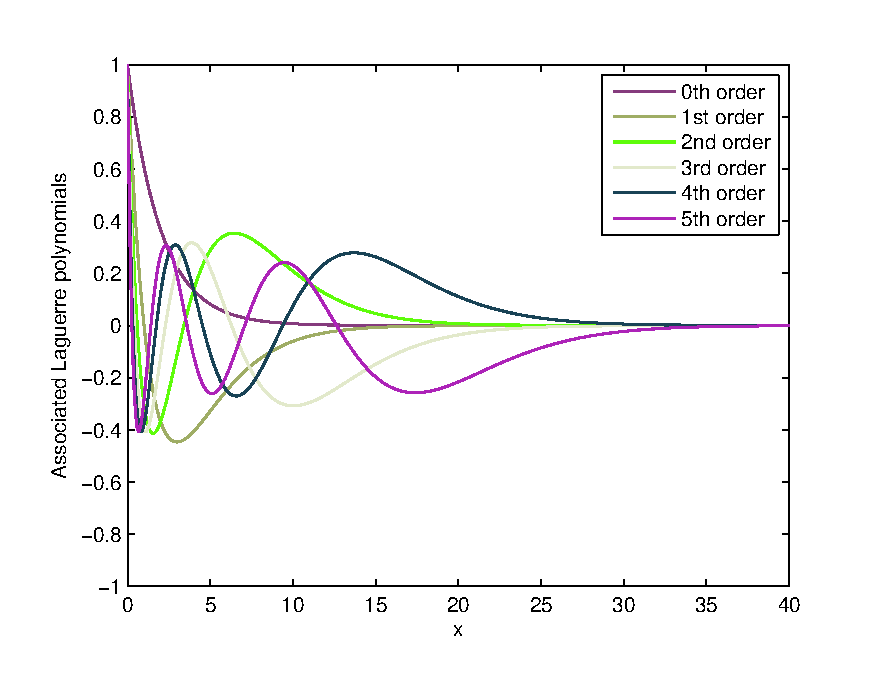
\includegraphics[width=.45\textwidth]{associated_laguerre.eps}}
  \caption{Associated Laguerre functions to the 5th order ($\alpha=5$ and $\alpha=5$).}
  \label{fig:associatedlaguerre}
\end{figure}

\section{Synthesised Data fitting}

\subsection{Least squares Laguerre fit}
We know that we can represent any function as a linear combination of the associated Laguerre functions. The coefficients of the functions in such combination can be easily calculated thanks to the orthogonality property under the inner product \ref{inner_product}.\\
We wish to optimize our fit in the least square sense, though. Writing down our function as $f(x)=a_0\psi_0(x)+a_1\psi_1(x)+\ldots$, we can expand the general definition for the least squares error as:
\begin{align}
e &= \int_{0}^{\infty} (f(x)-f_0(x))^2dx \\
  &= \int_{0}^{\infty} f^2 - 2 \int_{0}^{\infty} f f_0 dx + \int_{0}^{\infty} f_0^2 \\
  &= \int_{0}^{\infty} (a_0)^2(\psi_0)^2 + a_0a_1\psi_0\psi_1 + \ldots dx - 2 \int_{0}^{\infty} (a_0\psi_0(x)+a_1\psi_1(x)+\ldots)f_0 dx + constant \\
  &= (a_0^2+a_1^2+\ldots) - 2 \int_{0}^{\infty} (a_0\psi_0(x)+a_1\psi_1(x)+\ldots)f_0 dx + constant
\end{align}

\noindent And now optimizing for the coefficients:
\begin{equation}
\frac{\partial e}{\partial a_n} = 2a_n - 2 \int_{0}^{\infty} \psi_nf_0dx = 0
\end{equation}
so that indeed:
\begin{equation}
a_n = \int_{0}^{\infty} \psi_nf_0dx
\end{equation}
as suggested by the inner product definition quoted earlier(\ref{inner_product}), which proves that the Laguerre fit is such under the least squares sense.

\subsection{Sample data}
The sample fitting data set was generated using the supplied \textit{exp\_data.m} function.
The function generates a set of random complex numbers, scaled by the factor $sqrt(\sigma^2/2)$ and shifted by the mean $\mu$. Power of the dataset is then calculated by squaring the modulus of the generated values. \\
In order to plot the data, we generate a histogram with a prescribed number of bins which represent equally spaced intervals. The number of power data samples belonging to each interval is then calculated, with the whole dataset subsequently normalized to approximate a probability density function.

\begin{figure}
\centering
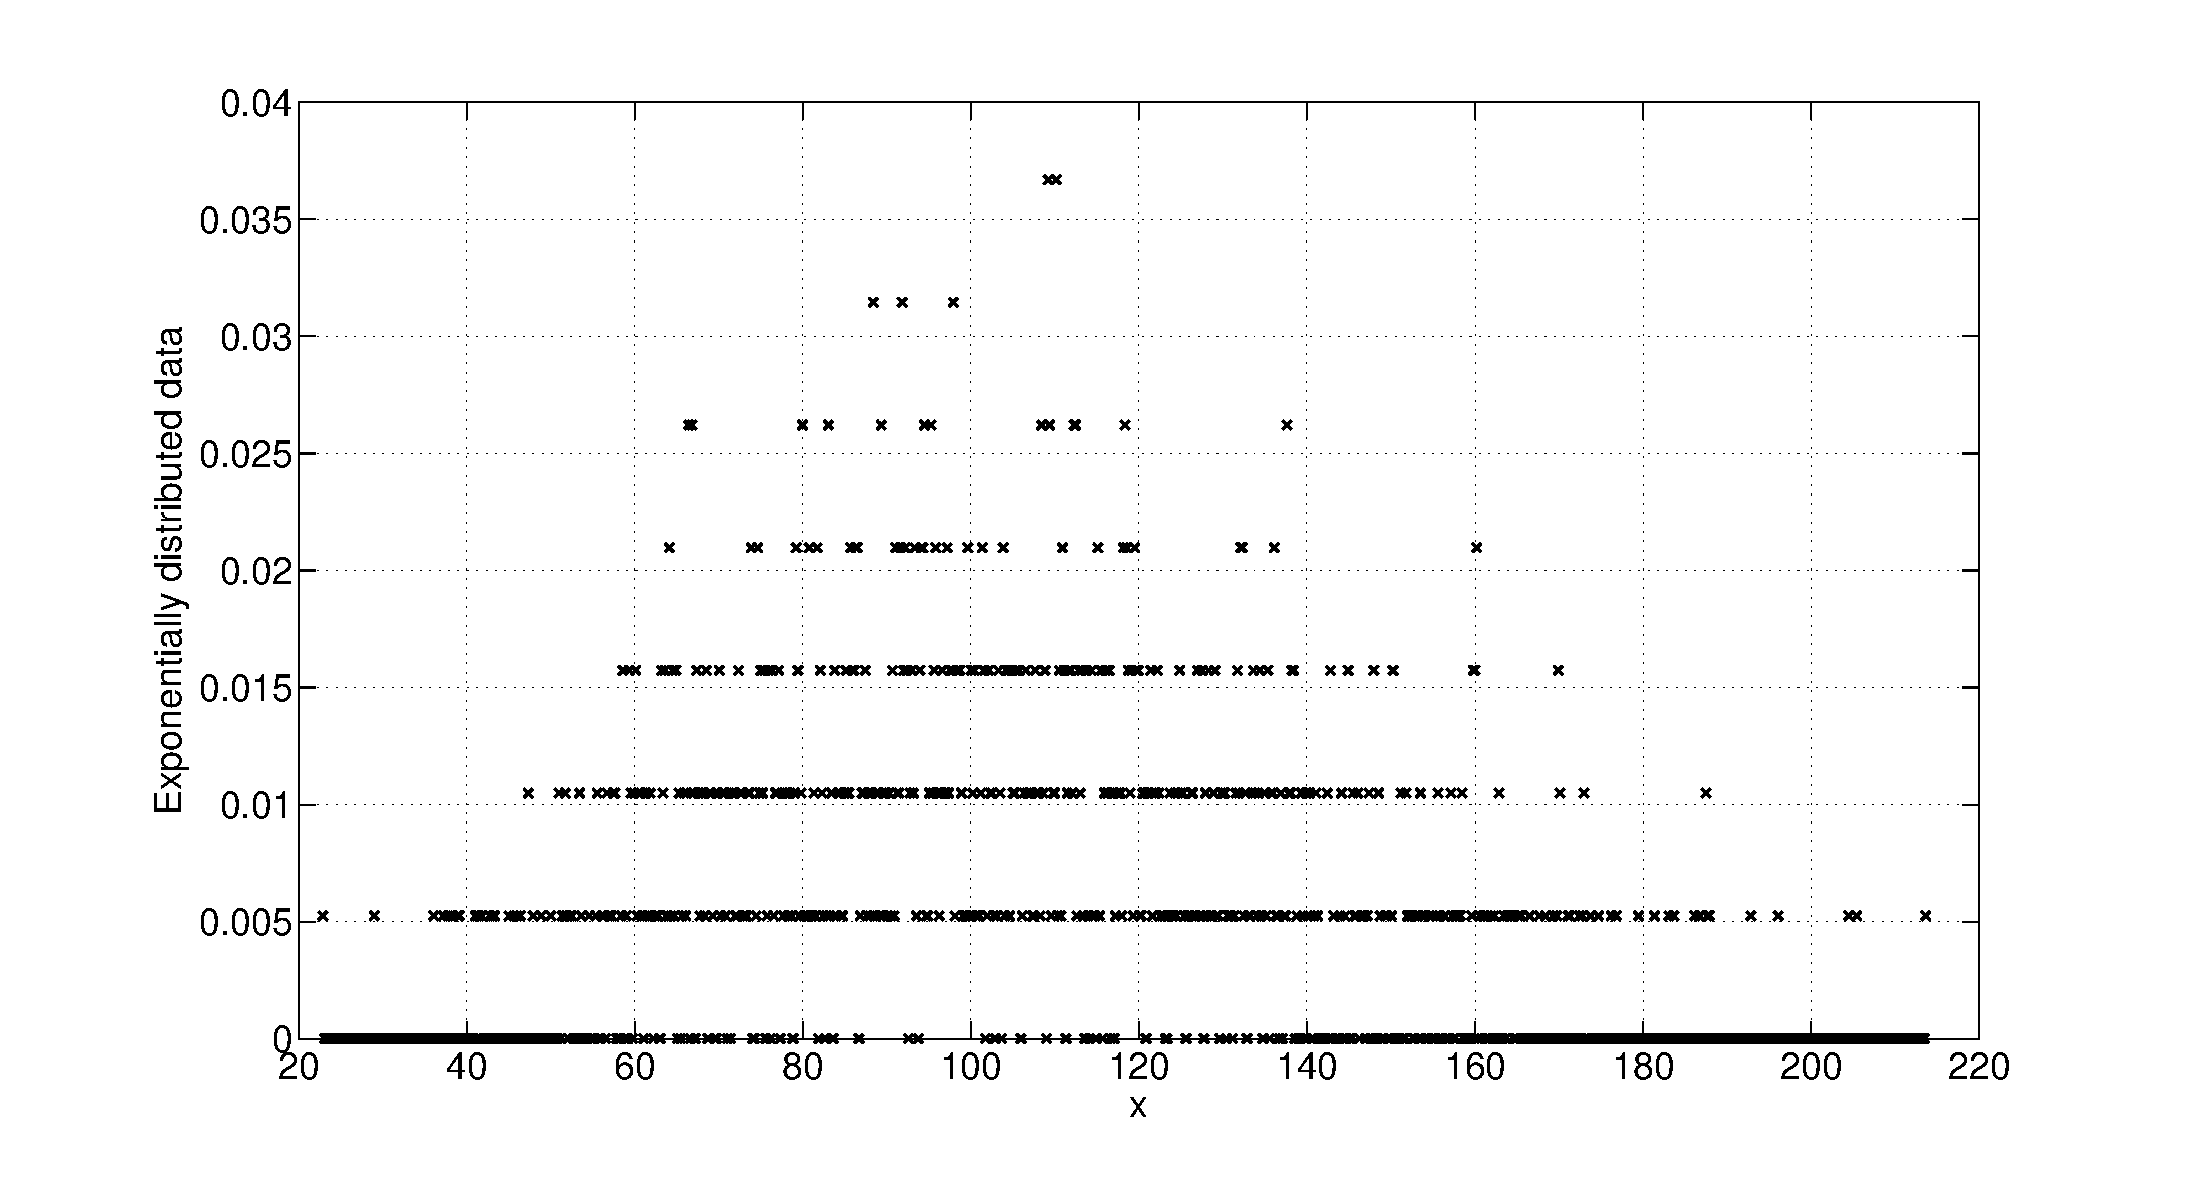
\includegraphics[width=0.8\textwidth]{exp_data.eps}
\caption{\label{fig:expdata}Exponentially distributed data.}
\end{figure}

\noindent The data shown in figure \ref{fig:expdata} was generated using $\sigma^2=5, \mu=10, n_{samples} = 1000, n_{bins} = 1000$. A distinctive feature of the set is "banding" of the data points, stemming from the fact that the non-normalized number of samples in a bin is always an integer, often the same for different bins. To obtain a less scattered graph the number of bins could thus be reduced.

\subsection{Basic Laguerre fit}
Having a sound dataset generated, the applicability of Laguerre function fitting could now be tested. The function \textit{laguerre\_fit.m} thus takes the four inputs:
\begin{itemize}
\item f0 - the function values
\item x - the domain for which the function values were generated
\item n - the highest desired order of the fitting Laguerre function
\item alpha - the $\alpha$ coefficient
\end{itemize}
and returns the \textbf{fitted data points} as an output.

\lstinputlisting[caption={laguerre\_fit.m},label={lst:laguerrefit},firstline=17, lastline=26]{../Matlab/FittingData/laguerre_fit.m}

\noindent The code listing \ref{lst:laguerrefit} numerically evaluates the inner product between the supplied dataset and the Laguerre function and then multiplies it by the data points of the said function.

\begin{figure}
\centering
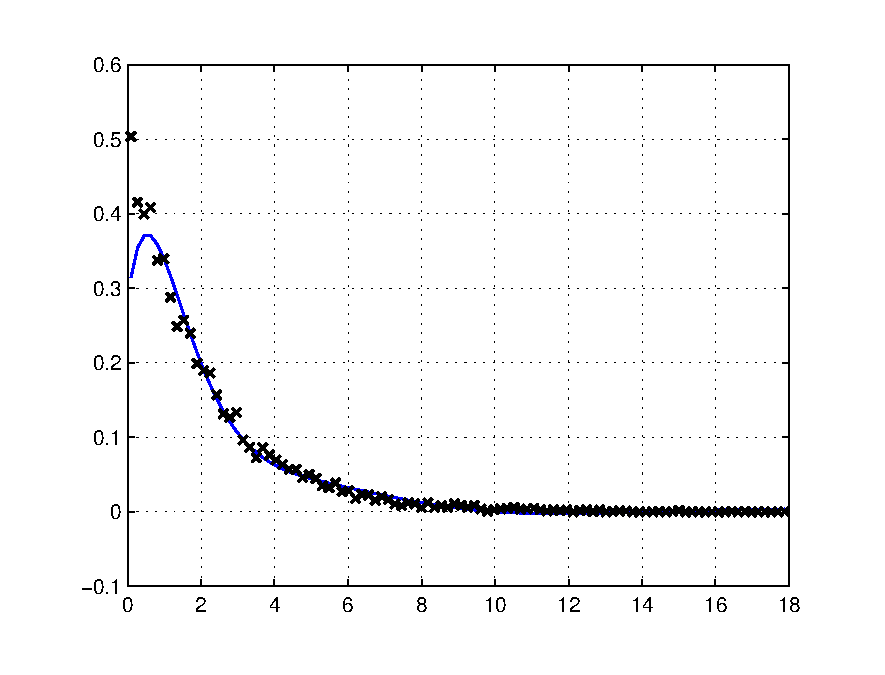
\includegraphics[width=0.5\textwidth]{basic_fit.eps}
\caption{\label{fig:basicfit}Basic 5th order, $\alpha=0$ Laguerre fit for $\sigma^2=2, \mu=0, n_{samples}=10^4, n_{bins}=100$.}
\end{figure}

\noindent Figure \ref{fig:basicfit} clearly shows that even though the fit further from the origin can be considered reasonable, it cannot cope with a sharp exponential increase near x=0.

\subsection{Parameterised fit comparison}
Realising the mathematical origin of the randomly scattered data gives us a way of testing the accuracy of the fit. Our generated data can be described by means of a random variable $X$ which is a sum of squares of two other random variables. Both have zero mean and an identical variance, which means that $X$ is chi-squared distributed. Since the probability density function of the chi-squared distribution is:
\begin{equation}
f(x) = \frac{1}{2^{n/2} \Gamma(n/2)}x^{n/2-1} e^{-x/2}, \quad x \in (0, \infty)
\end{equation}
where, in our case, the number of degrees of freeedom $n$, equals $2$, hence:
\begin{equation}
f(x) = \frac{1}{2} e^{-x/2}
\end{equation}

\noindent Given our definition of the associated Laguerre functions (eq. \ref{associated_laguerre_definition}), an $\alpha = 0$, 0th order fit should provide an exact match for the above pdf. To compare it to the expectation, we construct a parameterised fit of the form $f(x) = \frac{1}{\xi} e^{-x/\xi}$. The mean $\xi$ is estimated by using the fact that for a probability distribution function $f(x)$ the mean is $\xi = \int_{0}^{\infty} xf(x) dx$.

\begin{figure}[!h]
\centering
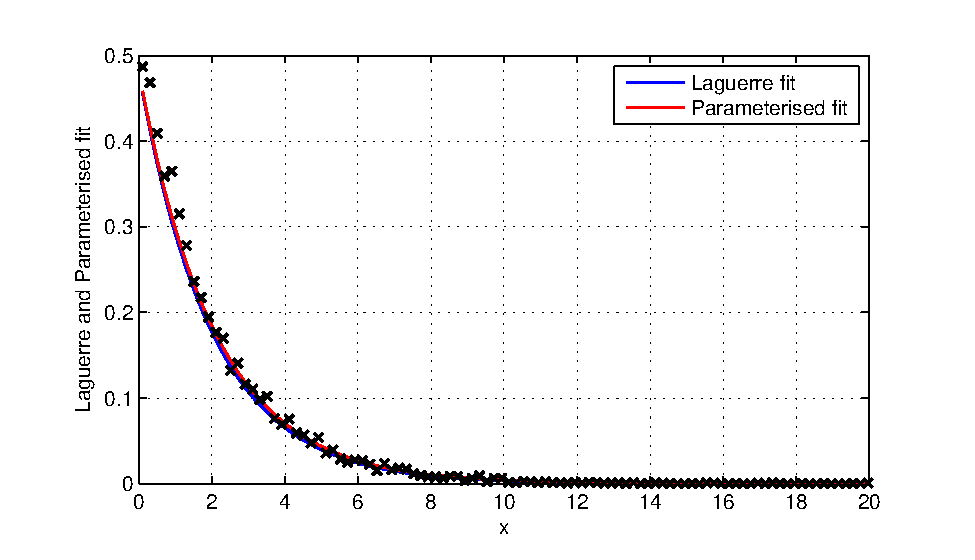
\includegraphics[width=0.8\textwidth]{laguerre_parameterised_fit.eps}
\caption{\label{fig:laguerreparemeterisedfit}Exponentially generated data, ideal parameterised fit(red) and the Laguerre fit (blue).}
\end{figure}

\noindent The error, in the least squares sense, between the Laguerre and parameterised fit (figure \ref{fig:laguerreparemeterisedfit}), was evaluated to be $2.30 \times 10^{-4}$. The parameterised fit seems to match the data more closely in the intermediate values of x, but the error between the two functions is insignificant - two orders of magnitude smaller than the largest function values.

\subsection{Difficult data}
It is clear that an orthonormal set of functions is best used for fitting in the range that it is defined. Fits for different orders and values of $\alpha$ are presented in figure \ref{fig:difficultfits}.

\begin{figure}[!ht]
  \centering
  \subfloat[][]{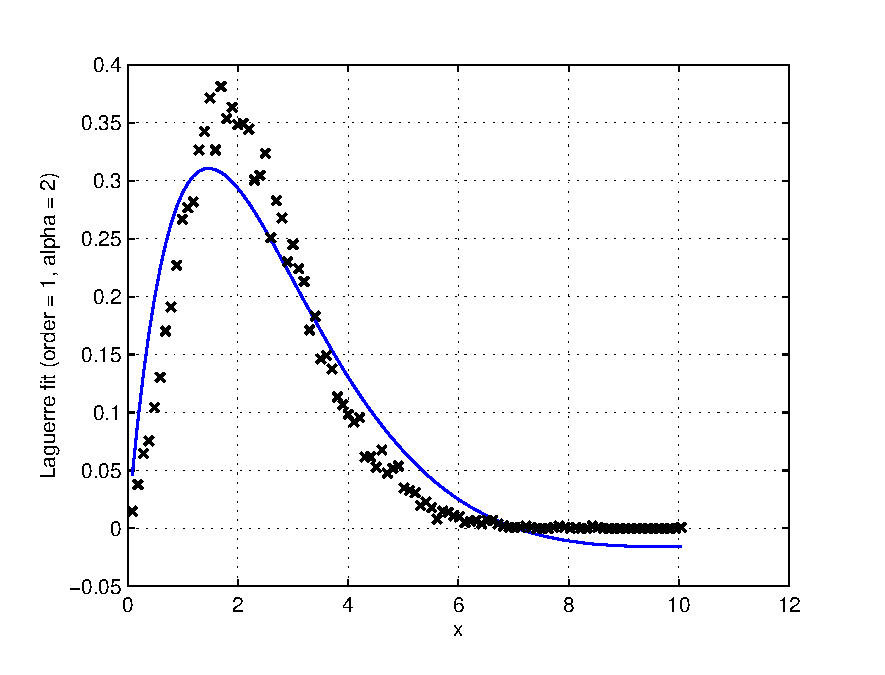
\includegraphics[width=.4\textwidth]{lfit_order1_alpha2.eps}}\quad
  \subfloat[][]{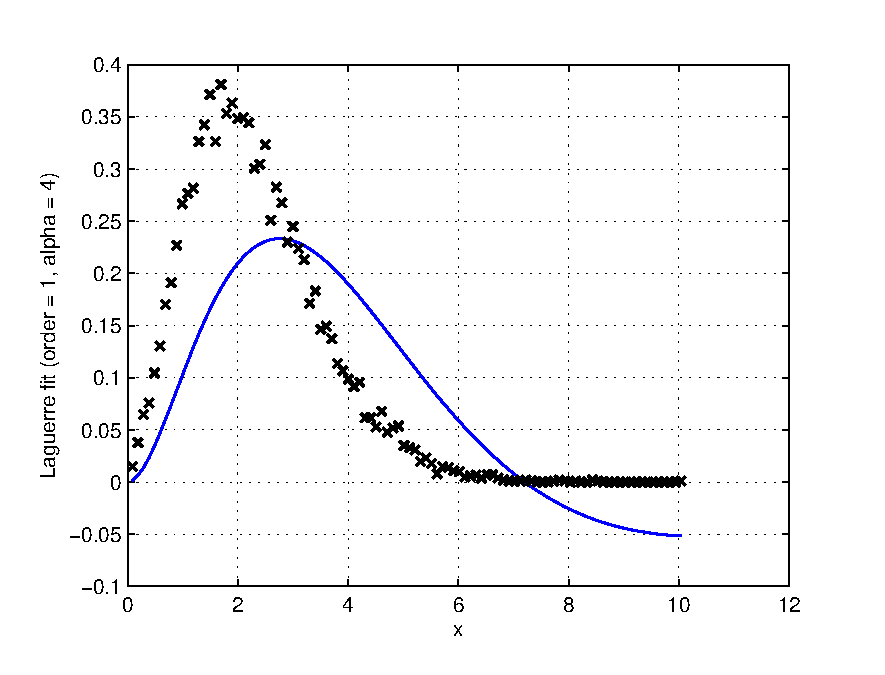
\includegraphics[width=.4\textwidth]{lfit_order1_alpha4.eps}}\\
  \subfloat[][]{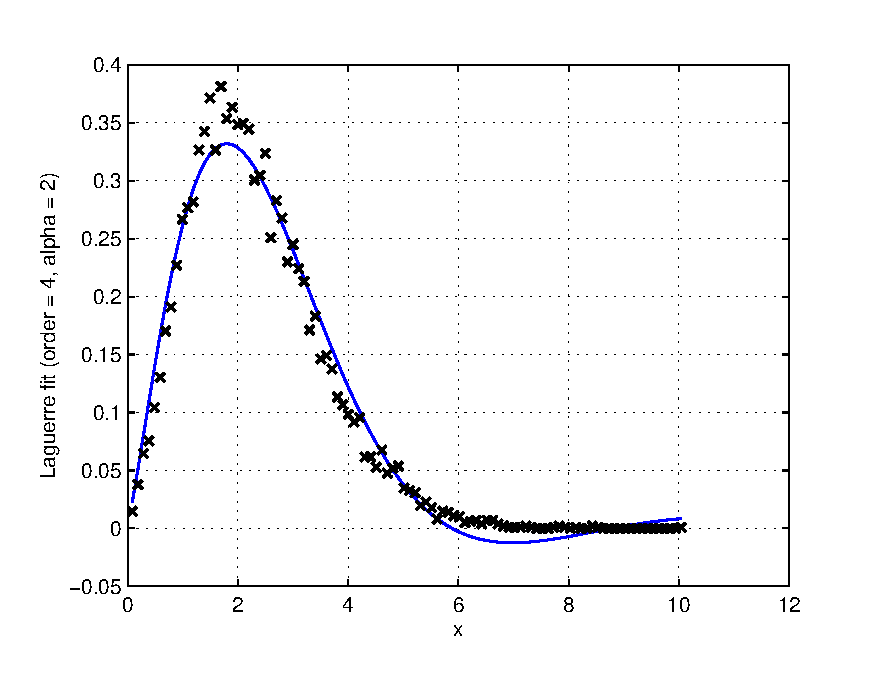
\includegraphics[width=.4\textwidth]{lfit_order4_alpha2.eps}}\quad
  \subfloat[][]{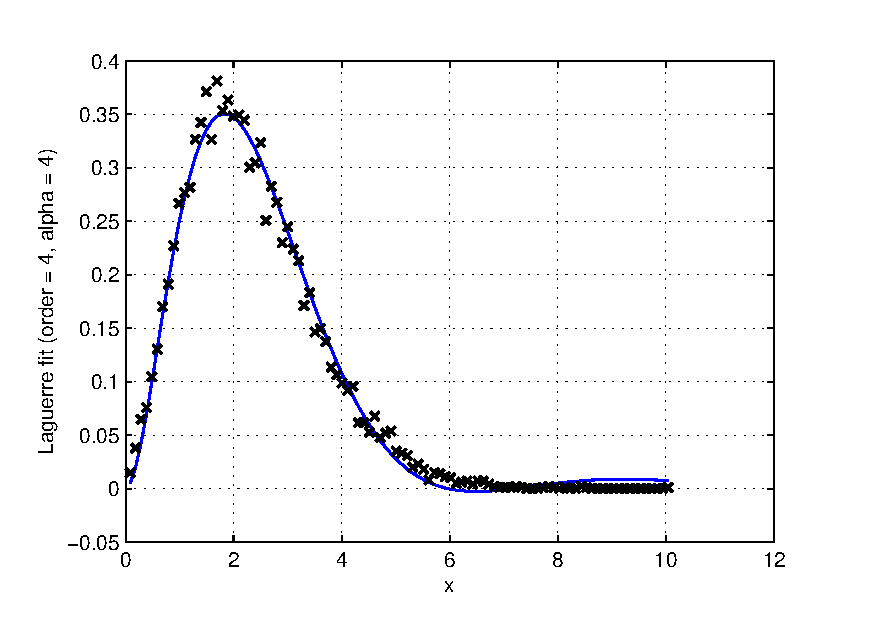
\includegraphics[width=.4\textwidth]{lfit_order4_alpha4.eps}}
  \caption{Laguerre fits of different orders and alpha parameters}
  \label{fig:difficultfits}
\end{figure}

\noindent As we can see, the higher order fits also provide a closer matching of the generated data. It is unclear from the figures, though, how alpha influences this accuracy - in case of the 0th order function bigger alpha deteriorated the fit, whereas for the 4th order it improved the fit noticeably. \\

\noindent It is worth noting that if the data is shifted even further, the Laguerre functions provide an even worse fit. Figure \ref{fig:poorfit} clearly shows that Laguerre fit is of nearly no use even for a mean of 5.

\begin{figure}[!h]
\centering
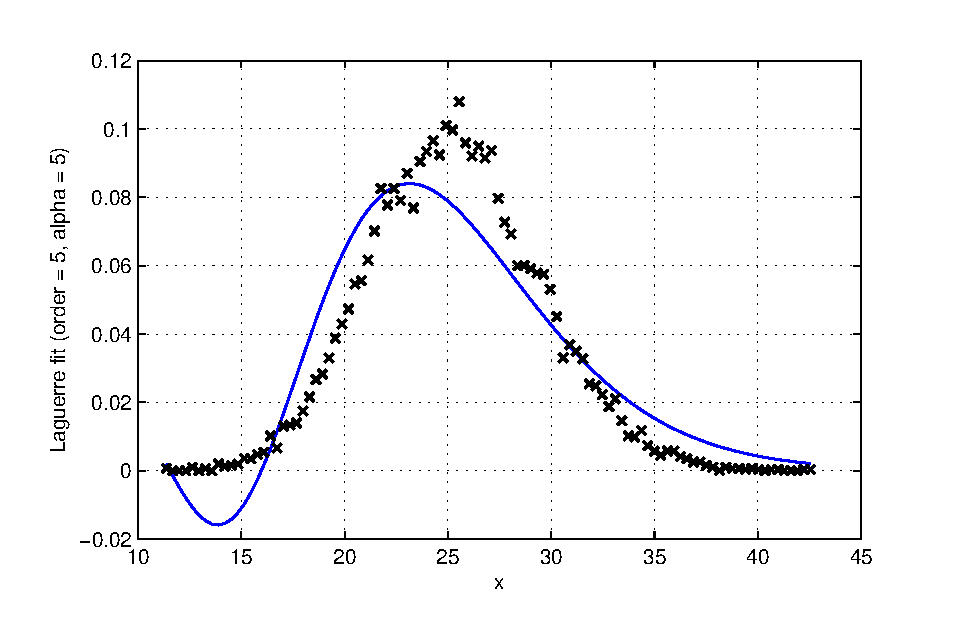
\includegraphics[width=0.8\textwidth]{poor_fit.eps}
\caption{\label{fig:poorfit}A fifth order Laguerre fit for $alpha=5$ with random data generated for $\sigma^2=1/3, \mu=5, n_{samples} = 10000, n_{bins} = 1000$}
\end{figure}

\subsection{Shifting and scaling}

Referring back to figure \ref{fig:associatedlaguerre}, the Laguerre polynomial values are defined on a range from $0$ to $~35$, nearing zero everywhere after. It is clear that even though the supplied dataset might be defined on a domain much larger than the desired Laguerre one, we can shift and scale it to match our needs. \\
\textbf{Shifting} is somewhat clear - since the Laguerre polynomials are best defined on the above interval, we should bring the dataset as close as possible to zero. This is done by subtracting the smallest x coordinate in the set from all the other values in the x range:
\begin{equation}
x^\prime(n) = x(n) - x(1)
\end{equation}
\textbf{Scaling} of the set is more subtle. To have a sound factor to optimize, we first scale the dataset to be defined on the range $(0,1)$ like:
\begin{equation}
x^\prime(n) = \frac{x(n) - x(1)}{x(n_{max}) - x(1)}
\end{equation}
and then scale it further by a factor $\lambda$:
\begin{equation}
x^\prime(n) = \lambda \times \frac{x(n) - x(1)}{x(n_{max}) - x(1)}
\end{equation}
Since the degree of the fit is arbitrarily chosen, the choice of $\lambda$ should be tailored to the particular domain of the value set as well as the Laguerre order. The other factor requiring optimisation is $\alpha$, whose value has been arbitrarily picked before, which is however crucial for the overall accuracy of the fit. \\

\noindent Both were simultaneously optimised using the fminsearch MATLAB function. \textbf{fminsearch} follows the Nelder-Mead method for finding a minimum of a function in a multidimensional space. The Nelder-Mead method, also called the amoeba algorithm, constructs a simplex in an n-dimensional space and tries to find an extremum of the given space. The algorithm iteratively and greedily replaces the "worst" point of the simplex through simple moves. Those are restricted to the reflection (through the centroid), expansion, contraction and reduction of the simplex. \\

\noindent In our case, the cost function requiring optimization was the least-squares error between the generated data and the fit. The implementation in listing \ref{lst:fittingerror} does exactly that - it first shifts and scales the domain, then computes the Laguerre fit and calculates the error.

\lstinputlisting[caption={fitting\_error.m},label={lst:fittingerror},firstline=23, lastline=34]{../Matlab/FittingData/fitting_error.m}

\noindent The error is then used in the laguerre\_optimal\_fit function which returns the values of the actual minimum-error fit. The fminsearch requires supplying the initial guesses for the parameter values, which were chosen to be 5 and 10 for alpha and lambda respectively. \\

\noindent The choice of the initial guesses was based on the empirical observations. The scaling parameter corresponds to the approximate middle of the interval for which the associated Laguerre polynomials are greater than 0.
Comparing the Associated Laguerre functions for $\alpha = 0$ and $\alpha = 5$ in figure \ref{fig:associatedlaguerre}, it is clear that the greater the alpha, the more right-shifted the maxima of the functions appear to be. That is why for the initial scaling factor of 10, an initial guess of $\alpha = 5$ is appropriate. It should be noted, however, that for $\alpha > 0$ the functions' values at the origin are 0. Hence for the datasets closer to the origin it might be beneficial to try fitting with $\alpha = 0$ and compare the difference between the fit errors for the two outcomes.

\lstinputlisting[caption={laguerre\_optimal\_fit.m},label={lst:laguerreoptimalfit},firstline=18, lastline=23]{../Matlab/FittingData/laguerre_optimal_fit.m}

\section{Real Data fitting}

\begin{figure}[!h]
\centering
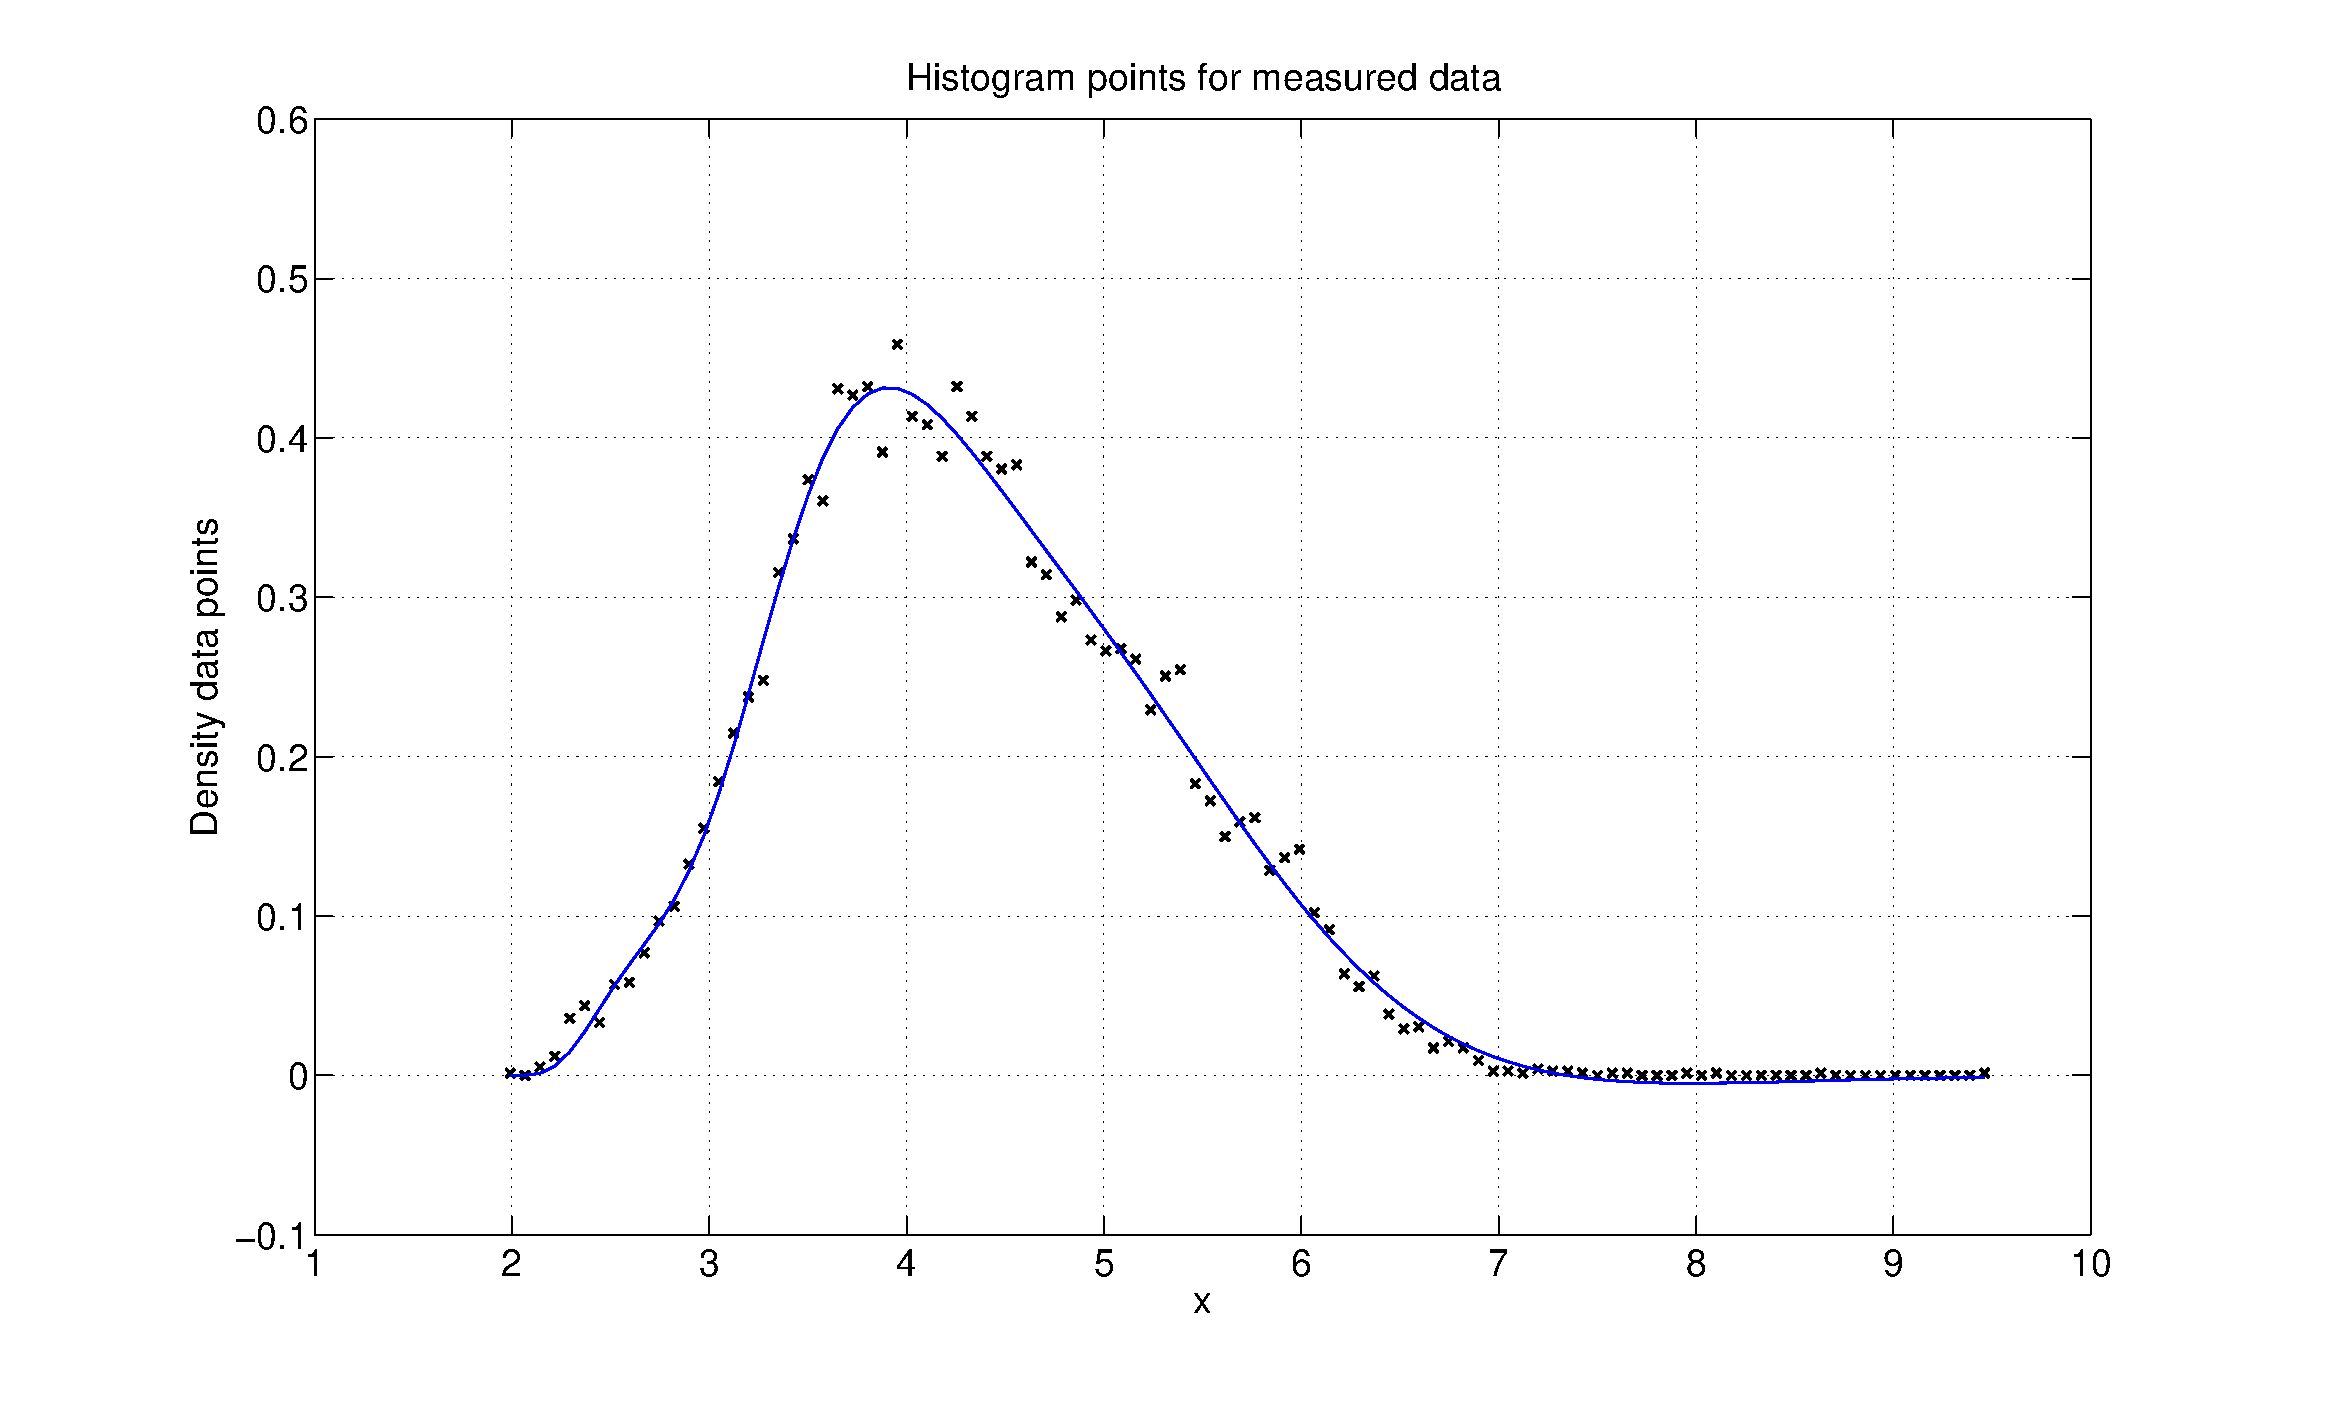
\includegraphics[width=0.8\textwidth]{real_data_fit.eps}
\caption{\label{fig:realdataset}A Laguerre fit to the measured dataset}
\end{figure}

\noindent As seen in figure \ref{fig:realdataset}, the fitting algorithm described above yields an excellent match between the measured data and the best fit line. The error between the two is $1.3 \times 10^{-3}$ for the 5th order fit.

\section{Conclusions}
The fitting procedure proved to be accurate for various datasets - close and far from the origin, both with high and low degree of scattering. The fitting proves to be extremely useful for statistical modelling of the obtained data. Computing the mode of the distribution corresponds to the position for which the power is maximum. The standard deviation will be useful for measuring the dispersion, or scattering, of the Wi-Fi signal. These can be used to design either more focused routers with a higher degree of penetration, or ones whose signal can spread through larger areas. Either way, more insight into spreading of the signal gives us a chance to design better, tailored communication systems.

\end{document}